\section{Computing closed trajectories with a flow graph}
\label{sec:flow-graph-algorithm-ch2021}

The quadratic program computes capacity by comparing possible facet orders
and weights. A second approach follows trajectories through the facets
themselves. In the relative interior of a facet, the contact-normalized
velocity is constant. Following a chosen facet direction carries a
point on an incoming two-dimensional section to an outgoing section by an
affine map. Composing these maps around a facet word produces a return map;
a fixed point gives a closed trajectory.

We use the local passage geometry of Chaidez and Hutchings~\cite{CH2021}.
The exhaustive search below is justified by the simple-minimizer theorem:
some capacity-minimizing trajectory uses each of its facet directions once.
It is therefore enough to search finitely many cyclic words, retaining the
conditions that make each passage possible. We state the regularity
hypotheses before the correctness theorem and discuss the rational
implementation after its proof.

\subsection{Affine tubes}
\label{subsec:flow-graph-algorithm-ch2021-definition}

Let
\[
  K=\{x\in\mathbb R^4:\langle a_i,x\rangle\leq1,
  \ i=1,\ldots,F\}
\]
be a bounded full-dimensional polytope with \(0\in\operatorname{int}K\), and
assume that all listed inequalities define genuine facets \(F_i\).  Put
\[
  R_i=2J_0a_i .
\]
As in Section~\ref{sec:generalized-reeb-orbits-polytopes}, a trajectory on
\(F_i\) with velocity \(R_i\) has action equal to its elapsed time.

For each ordered pair \((i,j)\) for which \(a_i,a_j\) are linearly
independent, choose affine coordinates
\[
  \psi_{ij}:\mathbb R^2\longrightarrow
  H_i\cap H_j,
  \qquad H_i=\{x:\langle a_i,x\rangle=1\},
\]
and let
\[
  P_{ij}=\{u\in\mathbb R^2:\psi_{ij}(u)\in K\}.
\]
The set \(P_{ij}\) is allowed to be empty or lower-dimensional.  Thus the
construction also permits a breakpoint to lie on additional facets; it does
not assume that every breakpoint lies in the relative interior of a
two-face.

Consider a passage from facet $F_p$ along $F_i$ to $F_n$, with three
distinct facet labels. We consider the case where the incoming direction
approaches $H_i$ and the direction along $F_i$ approaches $H_n$:
\[
  \langle R_p,a_i\rangle>0,
  \qquad
  \langle R_i,a_n\rangle>0.
\]
For \(x\in F_p\cap F_i\), the time at which the line
\(x+tR_i\) reaches \(H_n\) is
\begin{equation}\label{eq:fg-primitive-time}
  \tau_{pin}(x)
  =\frac{1-\langle a_n,x\rangle}{\langle a_n,R_i\rangle}.
\end{equation}
The denominator is positive.  Restrict the starting section to those points
for which \(x\in K\), \(x+\tau_{pin}(x)R_i\in K\), and
\(\tau_{pin}(x)\geq0\).  On this closed polygonal domain, the endpoint map
\[
  \varphi_{pin}(x)=x+\tau_{pin}(x)R_i
\]
and the action contribution \(\tau_{pin}\) are affine.  Convexity of \(K\)
ensures that the whole segment lies in \(K\cap H_i\).

We describe a tube by a closed starting polygon \(P\), an affine endpoint map
\(\Phi\), and an affine total-action function \(A\).  If
\((P_1,\Phi_1,A_1)\) and \((P_2,\Phi_2,A_2)\) are consecutive tubes in
matching coordinates, their concatenation is
\begin{equation}\label{eq:fg-tube-composition}
  \bigl(P_1\cap\Phi_1^{-1}(P_2),
  \ \Phi_2\circ\Phi_1,
  \ A_1+A_2\circ\Phi_1\bigr).
\end{equation}
Thus an empty intermediate intersection excludes every longer word containing
that partial tube.

A \emph{simple cyclic facet word} is a cyclic word
\(w=[s_1,\ldots,s_k]\) with distinct entries.  To close it, concatenate the
primitive tubes for
\[
  (s_1,\ldots,s_k,s_1,s_2).
\]
Each primitive consumes three consecutive labels: the first passage is
\((s_1,s_2,s_3)\), from \(H_{s_1}\cap H_{s_2}\) to
\(H_{s_2}\cap H_{s_3}\).  The appended labels make the last passage
\((s_k,s_1,s_2)\), returning to the initial section.
Write the resulting data as \((P_w,\Phi_w,A_w)\).  A point
\(u\in P_w\) is a closed search candidate precisely when
\(\Phi_w(u)=u\).  It represents the displayed word as a strict generalized
Reeb orbit precisely when every reconstructed segment time is positive.  In
that case its action is \(A_w(u)\).

\begin{lemma}[Tube semantics]\label{lem:flow-graph-tube-semantics}
For every simple cyclic word whose primitive denominators are positive, the
fixed points of \(\Phi_w\) in \(P_w\) are exactly its closed nonnegative-time
tube realizations.  The fixed points with all segment times positive are
exactly the strict closed generalized Reeb orbits represented by \(w\), and
their action is \(A_w\).
\end{lemma}

\begin{proof}
Equation~\eqref{eq:fg-primitive-time} gives the unique next breakpoint and
elapsed time for one passage.  The endpoint and the elapsed time are affine,
and the domain inequalities state exactly that the endpoints and the passage
belong to \(K\).  Formula~\eqref{eq:fg-tube-composition} says that two passages
can be concatenated exactly when their common breakpoint agrees; it also
composes their endpoint maps and adds their elapsed times.  Induction over the
word proves the assertion for the closed tube.  Its starting and ending
sections have the same coordinates, so closure is equivalent to
\(\Phi_w(u)=u\).  Finally, the closed tube was defined with nonnegative times,
whereas the active word omits zero-time passages and records only the
positive-duration pieces.  Thus the entire displayed word is active exactly
when every passage time is positive.  Since
\(\lambda_0(R_i)=1\) on \(F_i\), the sum of the elapsed times is the Reeb
action.
\end{proof}

\begin{example}[A return map on a two-dimensional section]
\label{ex:flow-graph-return-map}
Figure~\ref{fig:flow-graph-tube-sequence} follows the word
\(w=[1,2,4,5,3]\) on a six-facet polytope.  For this example we number the
facets from \(0\) to \(5\), as in the figure.  The normalized facet rows,
rounded here to four decimal places, are
\[
\begin{pmatrix}
-0.2091&-0.8088& 1.6079&-0.0729\\
 0.2405& 0.5222& 0.6397&-0.2308\\
-0.8794&-0.3786& 0.2356& 0.0382\\
 0.2108&-0.2660& 0.1605&-0.3711\\
-0.3527& 0.1313&-0.4414& 0.0589\\
-0.1226& 0.1707&-0.1480& 0.4331
\end{pmatrix}.
\]
The exact dyadic rows and all rational calculations for this example are
stored in
\path{experiments/dev-flow-graph/visualize-tube/flow-graph-f6-tube.json}
(the six-facet instance with seed 20260605 and attempt 3); see also
Section~\ref{sec:published-code-data}.
The rounded numbers below illustrate the calculation; the exact values decide
membership and closure.

Start on \(F_1\cap F_2\), immediately before the passage along \(F_2\).
A convenient affine chart uses the last two ambient coordinates:
\[
\psi_{12}(u,v)\simeq
\begin{pmatrix}-2.446722\\3.041760\\0\\0\end{pmatrix}
+u\begin{pmatrix}0.991996\\-1.681765\\1\\0\end{pmatrix}
+v\begin{pmatrix}-0.183156\\0.526320\\0\\1\end{pmatrix}.
\]
The five passages take this section successively to
\(F_2\cap F_4\), \(F_4\cap F_5\), \(F_5\cap F_3\),
\(F_3\cap F_1\), and back to \(F_1\cap F_2\).
Composing their affine maps gives
\[
\Phi_w(u,v)\simeq
\begin{pmatrix}-1.601002&1.364891\\4.482887&-4.446374\end{pmatrix}
\binom uv+
\binom{1.626615}{-1.821973},
\]
\[
A_w(u,v)\simeq36.063319+6.721729u-6.397030v.
\]
The fixed point is \((u,v)\simeq(0.791856,0.317243)\).  It belongs to the
closed tube, and its five passage times are approximately
\[
  0.538394,\quad5.134160,\quad14.681452,\quad16.367140,\quad2.635397.
\]
They are all positive and sum to the orbit's action, approximately
\(39.356542\).  Thus the fixed-point calculation produces a closed orbit.
Finding the capacity still requires comparison with the other words.
\end{example}

\begin{figure}[htbp]
  \centering
  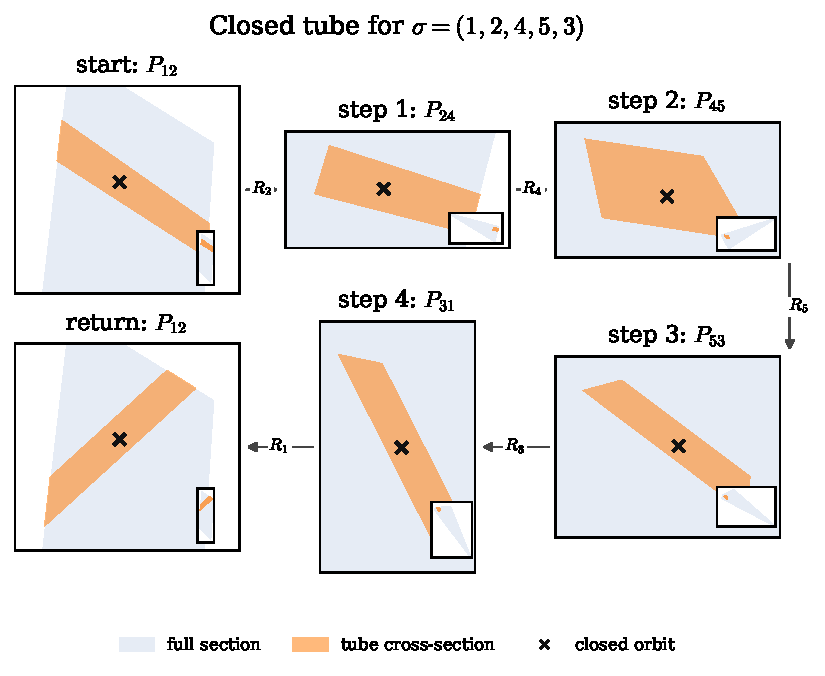
\includegraphics[width=\linewidth]{figures/flow-graph/flow-graph-f6-tube-sequence.pdf}
  \caption{The five passages of Example~\ref{ex:flow-graph-return-map}.
    The colored polygons are the successive sections of the tube; each inset
    locates the displayed region in the full facet-pair section.  The black
    cross follows the closed orbit.  Each panel uses a Euclidean-orthonormal
    frame, so its coordinates differ from the affine chart used in the text.
    The start and return panels share a frame and scale: closure returns the
    cross to the same position.}
  \label{fig:flow-graph-tube-sequence}
\end{figure}

\FloatBarrier
\subsection{Exhaustive search and correctness}
\label{subsec:flow-graph-algorithm-ch2021-correctness}

The fixed-point calculation is simplest when every surviving return map has
a unique fixed point.  The following hypotheses make this precise and also
justify the two pruning rules used in the search.

\begin{definition}[Flow-graph regular presentation]
\label{def:flow-graph-regular-presentation}
The facet presentation above is \emph{flow-graph regular} if:
\begin{enumerate}
  \item for distinct \(i,j\),
    \(F_i\cap F_j\ne\varnothing\) implies
    \(\omega_0(a_i,a_j)\ne0\);
  \item every sublist of at most four of the vectors
    \(a_1,\ldots,a_F\) is linearly independent; and
  \item for every simple cyclic word of length at least five which survives
    the facet-intersection and positive-transition tests and has nonempty
    closed tube domain, the linear part \(M_w\) of \(\Phi_w\) satisfies
    \(\det(I-M_w)\ne0\).
\end{enumerate}
The last condition is called \emph{finite-orbit regularity}.
\end{definition}

\begin{algorithm}[Idealized exhaustive flow-graph search]
\label{alg:idealized-exhaustive-flow-graph-search}
Enumerate every simple cyclic facet word once.  For each word:
\begin{enumerate}
  \item discard it if an adjacent facet intersection is empty or an adjacent
    transition sign is not positive;
  \item discard it if its length is at most four: under the regularity
    hypothesis, these facet directions are linearly independent and cannot
    form a closed positive-time path;
  \item construct its closed tube \((P_w,\Phi_w,A_w)\); discard the word
    if \(P_w=\varnothing\), and otherwise solve \(\Phi_w(u)=u\);
  \item reject a singular fixed-point equation as outside the regular case,
    and otherwise record the unique solution only if it lies in \(P_w\) and
    every reconstructed segment time is positive.
\end{enumerate}
Return the least positive recorded action.
\end{algorithm}

We justify both pruning steps.  If a strict trajectory changes from \(R_i\) to
\(R_j\) at \(x\in F_i\cap F_j\), then the inequalities
for \(K\) immediately before the breakpoint give
\[
  \langle a_j,R_i\rangle\geq0.
\]
The first condition in
Definition~\ref{def:flow-graph-regular-presentation} excludes equality.  Thus
every trajectory transition has the positive sign used by the search, even
when \(x\) lies on additional facets.  Second, a strict closed orbit with
active word \((s_1,\ldots,s_k)\) satisfies
\[
  \sum_{r=1}^k\tau_rR_{s_r}=0,
  \qquad \tau_r>0.
\]
If \(k\leq4\), this contradicts the linear independence in condition~2.

\begin{theorem}[Idealized real-arithmetic flow-graph correctness]
\label{thm:exact-flow-graph-correctness}
Let \(K\subset\mathbb R^4\) be a bounded full-dimensional convex polytope
with \(0\in\operatorname{int}K\), equipped with a flow-graph regular ordered
normalized irredundant facet presentation.  Then the finite procedure in
Algorithm~\ref{alg:idealized-exhaustive-flow-graph-search}, with its algebraic
and order operations performed exactly over \(\mathbb R\), returns
\[
  c_{\mathrm{EHZ}}(K).
\]
\end{theorem}

\begin{proof}
There are finitely many simple cyclic words.  By
Lemma~\ref{lem:flow-graph-tube-semantics}, every recorded point is a strict
closed generalized Reeb orbit with the recorded action.  The strict
transition-sign argument and the short-word linear-independence argument above
show that neither pruning rule can remove such an orbit.  Empty tubes contain
no orbit and are discarded before
solving a fixed-point equation. Finite-orbit regularity makes every remaining
fixed-point equation nonsingular, so no long word reaches the rejection
branch and each word has at most one fixed point.

By Theorem~\ref{thm:generalized-reeb-simple-minimizer}, a capacity-minimizing
orbit can be chosen with an active cyclic word in which every used facet
direction occurs in one positive-duration interval.  Its breakpoints lie in
the corresponding facet-pair sections, its transitions have the required
positive signs, and its passages satisfy the primitive tube equations.
Lemma~\ref{lem:flow-graph-tube-semantics} therefore represents it by a strict
fixed point with action \(c_{\mathrm{EHZ}}(K)\).  The returned minimum is no
larger than this action, while soundness of every recorded orbit makes it no
smaller.
\end{proof}

\begin{corollary}[Exact rational-arithmetic flow-graph correctness]
\label{cor:rational-flow-graph-correctness}
Under the hypotheses of
Theorem~\ref{thm:exact-flow-graph-correctness}, assume in addition that
\(a_i\in\mathbb Q^4\) for every facet row.  Then rational affine coordinates
can be chosen for every facet-pair plane, and
Algorithm~\ref{alg:idealized-exhaustive-flow-graph-search} is a finite exact
rational-arithmetic algorithm returning \(c_{\mathrm{EHZ}}(K)\).
\end{corollary}

\begin{proof}
Rational Gaussian elimination gives a rational base point and basis for every
facet-pair plane.  In these coordinates, the section inequalities, primitive
times and maps, tube intersections and compositions, and nonsingular
fixed-point systems all have rational coefficients.  Their feasibility, signs,
solutions, and action comparisons can therefore be decided in exact rational
arithmetic.  The conclusion follows from
Theorem~\ref{thm:exact-flow-graph-correctness}.
\end{proof}

\subsection{Why the regular class is generic}
\label{subsec:flow-graph-algorithm-ch2021-genericity}

The regularity assumptions are explicit algebraic nonvanishing conditions.
For fixed facet count there are only finitely many of them.  Pairwise
symplectic degeneracy and short-word dependence are ordinary polynomial
conditions.  The only non-immediate point is that the long-word determinant is
not the zero rational function.

When all cyclic primitive denominators of a word are nonzero, let
\(M_w^{\mathrm{alg}}\) denote the composition of the primitive linear maps,
regardless of their signs or whether the geometric tube domain is nonempty.
For a searched tube, this is the linear part \(M_w\) of its affine return map.

\begin{proposition}[Presentation-chamber genericity]
\label{prop:flow-graph-presentation-chamber-genericity}
Fix \(F\), and let \(\mathcal C\subset(\mathbb R^4)^F\) be a nonempty
Euclidean-open set of ordered normalized dual-row lists defining bounded
full-dimensional polytopes with \(0\) in the interior and all \(F\)
inequalities irredundant.  An open dense subset of \(\mathcal C\) satisfies
the stronger conditions
\begin{enumerate}
  \item \(\omega_0(a_i,a_j)\ne0\) for every \(i\ne j\);
  \item every sublist of at most four rows is linearly independent; and
  \item \(\det(I-M_w^{\mathrm{alg}})\ne0\) for every simple cyclic word \(w\)
    of length at least five.
\end{enumerate}
Consequently every presentation in this subset satisfies
Theorem~\ref{thm:exact-flow-graph-correctness}, and every rational presentation
in it satisfies Corollary~\ref{cor:rational-flow-graph-correctness}.
\end{proposition}

\begin{proof}
The first two families are finite collections of nonzero polynomial
conditions.  Fix a simple word \(w=(s_1,\ldots,s_k)\), and write
\(b_r=a_{s_r}\), with cyclic indices.  For its nonvanishing argument the
\(k\) rows vary independently in the affine space
\(X_k=(\mathbb R^4)^k\).  Let \(D_k\subset X_k\) be the set where all
cyclic pairings \(\langle b_{r+2},2J_0b_{r+1}\rangle\) are nonzero.
They imply that every adjacent pair is linearly independent, so
\(V_{pi}=\ker b_p\cap\ker b_i\) is a two-dimensional section direction.
The primitive linear map is
\[
  D_{pin}:V_{pi}\longrightarrow V_{in},\qquad
  D_{pin}\xi=\xi-
  \frac{\langle b_n,\xi\rangle}{\langle b_n,2J_0b_i\rangle}
  2J_0b_i.
\]
Choosing a nonzero coordinate minor for each adjacent pair gives bases for
these planes that depend rationally on the rows.  Thus the return-map
determinant is rational on each such chart; its values agree on overlaps
because the determinant is independent of the starting basis.

We first record an identity that permits witnesses of arbitrary length.
Here \(x,A,B,y\) denote row labels, and \(R_A=2J_0b_A\).
Whenever the displayed primitive denominators are nonzero,
\[
  D_{BAy}D_{ABA}D_{xAB}=D_{xAy}
  \quad\hbox{on }V_{xA}.
\]
Indeed, for \(\xi\in V_{xA}\), put
\(t=\langle b_B,\xi\rangle/\langle b_B,R_A\rangle\) and
\(\eta=\xi-tR_A\).  Then \(\eta\in V_{AB}\), so
\(D_{ABA}\eta=\eta\), since \(\langle b_A,\eta\rangle=0\).
The last passage gives
\[
 D_{BAy}\eta
 =\xi-tR_A-
 \frac{\langle b_y,\xi\rangle-t\langle b_y,R_A\rangle}
      {\langle b_y,R_A\rangle}R_A
 =D_{xAy}\xi.
\]
Both sides have domain \(V_{xA}\) and target \(V_{Ay}\).  Thus replacing
\((x,A,B,A,y)\) by \((x,A,y)\) preserves the entire return map when the
cyclic cut is taken at this unchanged incoming section.

Now specialize the row variables to
\[
\begin{aligned}
 A&=(2,3,-4,-3),& B&=(0,1,2,-1),& C&=(-4,-3,0,-1),\\
 D&=(4,-1,1,1),& E&=(-4,2,-4,-4).
\end{aligned}
\]
The required pairings are all nonzero, as the following complete table
shows (reversing a pair reverses its sign):
\[
\begin{array}{c|rrrrrrrrrr}
 pq&AB&AC&AD&AE&BC&BD&BE&CD&CE&DE\\ \hline
 \langle q,2J_0p\rangle&8&-56&36&-60&8&-16&12&-16&60&-20
\end{array}
\]
Direct substitution into the primitive formula gives
\[
  \det(I-M_{ABCDE}^{\mathrm{alg}})=-\frac{10643}{600},
  \qquad
  \det(I-M_{ACDE}^{\mathrm{alg}})=\frac1{168}.
\]
For odd length \(k=2m+3\), \(m\geq1\), specialize to
\((A,B)^m,C,D,E\).  Repeatedly contracting \((E,A,B,A,B)\) reduces this
tuple to \((A,B,C,D,E)\).  For even length \(k=2m+4\), \(m\geq1\), use
\((A,B)^m,A,C,D,E\).  The same contractions reduce it to
\((A,B,A,C,D,E)\), and contracting \((E,A,B,A,C)\) leaves
\((A,C,D,E)\).  Taking the cyclic cut at \(V_{EA}\) makes each contraction
preserve the return map.  Changing the cut does not change its determinant:
each primitive is invertible, with inverse obtained by projecting back along
the same \(R_i\), so cyclic return maps are conjugate.

These are algebraic specializations of independent row variables; the
repeated vectors do not describe simple searched words or irredundant
presentations.  They are legitimate evaluations of the rational function
on \(D_k\), and suffice to show that it is not identically zero for any
\(k\geq5\).  They also show that \(D_k\) is nonempty.  As a nonempty
Zariski-open subset of the irreducible affine space \(X_k\), it meets every
nonempty coordinate-minor chart in a dense set.  A nonzero rational function
cannot vanish identically on such a chart.  Its nonzero locus is therefore
open dense in \(D_k\), and hence in \(X_k\), since the excluded denominators
are nonzero polynomials.

For fixed \(F\), selecting the rows of a simple word pulls this open dense
condition back to \((\mathbb R^4)^F\): the remaining rows are free variables.
There are only finitely many simple words and sublists.  Intersecting their
open dense nonvanishing loci, and then the Euclidean-open chamber
\(\mathcal C\), preserves density.  The all-pairs condition is stronger than
the nonempty-pair condition in
Definition~\ref{def:flow-graph-regular-presentation}, and the remaining
conditions imply finite-orbit regularity.
\end{proof}

This is chamber-relative genericity for ordered normalized irredundant
presentations.  It is not the conjectural CH2021 claim that generic polytopes
have no Type~2 orbit below an action bound.

\subsection{Relation to CH2021}
\label{subsec:flow-graph-algorithm-ch2021-relation-to-ch2021}

Chaidez--Hutchings study a finite model that compares Reeb dynamics on a
four-dimensional polytope with Reeb dynamics on its smoothings
\cite{CH2021}.  Their setting and proof route differ from the general
Haim--Kislev formula.  They assume that the polytope is \emph{symplectic}; in
particular, its two-faces are not Lagrangian, so the relevant combinatorial
Reeb direction on each two-face is one-dimensional.

A Chaidez--Hutchings combinatorial Reeb orbit is a cyclic sequence of oriented
line segments in the boundary.  Their symplectic flow graph records the orbits
which avoid the one-skeleton: its vertices are open two-faces, an edge is a
Reeb passage through a three-face, and periodic graph orbits correspond to
these Type~1 combinatorial Reeb orbits with the same action
\cite[Proposition~2.14]{CH2021}.  Their smoothing theory relates this model to
Reeb orbits on smooth convex approximations and yields a capacity formula
involving Type~1 and Type~2 combinatorial orbits
\cite[Theorems~1.11 and~1.12, Corollary~1.15]{CH2021}.

The exact algorithm developed here uses part of the same local geometry but a
different global argument.  Its nodes are closed facet-pair sections, and it
searches simple facet words whose affine return maps have fixed points.  The
simple-minimizer theorem supplies completeness on the stated regular class.
Consequently this algorithm neither implements the CH2021 rotation pruning nor
imports the Type~1/Type~2/Type~3 classification as its capacity proof.  In
particular, an action cutoff alone would not control arbitrarily long helical
combinatorial words in the CH2021 model; the finite search here instead comes
from simple words with no repeated facet direction.


\subsection{Scope and rational implementation}
\label{subsec:flow-graph-algorithm-ch2021-implementation}

The regularity hypotheses exclude some important structured examples.
In a Lagrangian polygon product, all facet normals from either factor lie in a
two-dimensional subspace.  Any three of them are linearly dependent, violating
condition~2 of Definition~\ref{def:flow-graph-regular-presentation}.
The genericity proposition therefore does not make this algorithm applicable
to the products studied later in the thesis.  The product quadratic program
of Section~\ref{sec:quadratic-program-algorithm-hk2019} provides a separate method
for those bodies.

The rational implementation follows the construction above: it enumerates
simple directed cycles with positive transitions, intersects and composes
affine tubes, and reconstructs the segment times at a return-map fixed point.
It assumes a bounded, irredundant rational facet presentation in dimension
four, with correct facet-incidence and symplectic-sign matrices supplied by
the caller.  These are input requirements, not conclusions of the tube search.
It checks short-word independence and rejects a nonempty facet pair with zero
symplectic pairing.  A singular fixed-point equation is harmless if it is
inconsistent or if its fixed set misses the tube; otherwise the implementation
reports an unsupported case.

On selected deterministic five-, six-, and seven-facet examples, this search
agrees with the certified quadratic-program capacity computation.  The tests
also exercise tube composition, positive-time reconstruction, and unsupported
inputs.  These comparisons check the correspondence between the rational
program and the theorem on particular inputs.  They do not establish a
performance advantage over the quadratic program; no common-input benchmark
is claimed here.\footnote{The exact search and its regression tests are in
\path{crates/symplectic/src/algorithms/flow_graph/exact_search.rs};
the worked example and its input are in
\path{experiments/dev-flow-graph/visualize-tube/}.}
